% -*- root: ../Manual.tex -*-
\chapter{\LaTeX\ avanzado}
\label{chap:LaTeXAvanzado}

Una vez que ya nos manejamos con las cosas básicas de \LaTeX, vamos a pasar a cosas más avanzadas, como las etiquetas, índices, marcos y Tikz. También veremos parte de desarrollo de paquetes y clases de \LaTeX: cómo crear comandos y entornos y modificarlos para que hagan lo que nosotros queremos. Para eso, antes veremos cómo funciona exactamente \LaTeX, que nos ayudará a la hora de entender por qué tenemos que hacer ciertas cosas, como compilar dos veces, o qué es lo que puede estar fallando cuando algo no funciona.

\section{¿Cómo funciona \LaTeX?}
\label{sec:FuncionamientoLaTeX}

El capítulo anterior pretendía ser un tutorial básico de \LaTeX, para que podamos ponernos a escribir rápidamente. Pero para avanzar, creo que es importante saber cómo funciona este sistema, más que nada para entender de dónde salen los errores y saber exactamente qué es lo que estamos haciendo. Además, como curiosidad informática tampoco viene nada mal.

Para ser precisos, más que de \LaTeX\ deberíamos hablar de \TeX, que es el ``núcleo'' escrito por Donald Knuth. Este núcleo es un compilador que, a grandes rasgos, tiene dos fases: la de expansión y la de compilación.

Cuando compilamos un documento para generar un PDF, lo que va haciendo \TeX\ es ir leyéndolo carácter a carácter, e ir traduciéndolo. Los caracteres normales se pasan sin modificar, y los comandos (los que empiezan por \textbackslash, como \verb|\textbf|) se expanden.

La expansión de un comando no es más que sustituirlo por su definición sustituyendo los argumentos. Por ejemplo, yo puedo definir el comando \verb|\vector|, que recibe un argumento (denotado por \verb|#1|) y que se expande como \verb|$\mathbf{#1}$|. Así, cuando \TeX\ encuentre \verb|\vector{a}| lo sustituirá por \verb|$\mathbf{a}$|. Este proceso se va realizando de forma recursiva: cuando el compilador expande un comando y se encuentra que la expansión ha metido más comandos, los expande a ellos también. Todo esto se hace en orden de izquierda a derecha.

Así, comando a comando, \TeX\ va expandiendo el documento hasta llegar a la forma más básica, que son los comandos primitivos de \TeX, que simplemente dicen cosas tan de bajo nivel ``añade este carácter a la línea'' o ``ahora usa esta fuente''. Con esos comandos, \TeX\ va decidiendo cómo va a ser la estructura del PDF que va a generar (los saltos de línea o de página, o la colocación de las imágenes, por ejemplo).

Finalmente, esa información se pasa a la ``segunda etapa'' de \TeX, que transforma esos comandos primitivos en un formato estándar para un documento que nosotros podamos visualizar: normalmente es PDF, pero también pueden ser otros como DVI.

La parte específica de \LaTeX\ consiste en comandos adicionales que facilitan la vida al usuario, pero a grandes rasgos el proceso de compilación es el mismo.

En la práctica, hay algunas cosas algo más complicadas, pero básicamente así funciona \LaTeX. Lo primero que leerá del documento será el \verb|\documentclass|, que le dirá qué archivo base cargar: ese archivo cargará los comandos de \LaTeX\ básicos y prepará el documento (tipo de fuente, márgenes, papel, etc). Después, las sentencias \verb|\usepackage| cargarán otros documentos con más macros y comandos, y en cuanto empiece el documento con \verb|\begin{document}| el compilador empezará a procesar todos esos caracteres y comandos escritos, expandiendo estos últimos hasta llegar a las instrucciones primitivas para mostrar tu PDF.

\paragraph{¿Esto es importante?} Algo sí, más que nada porque nos explica de dónde salen dos tipos problemas muy habituales. El primero son los relacionados con la expansión de comandos: \LaTeX\ no es como un lenguaje de programación donde primero se evalúan los argumentos y luego se le pasan a la función. Aquí es al revés: primero se desarrolla la función (el comando) y luego se procesan los argumentos. Y si en algún momento algo no cuadra (cosa probable) la compilación falla.

La otra cuestión es algo que no hemos dicho explícitamente, pero que se puede ver: \TeX\ es un sistema de una sola pasada. Lee el fichero y va procesando según le llega, pero en ningún momento mira hacia atrás ni hacia delante\footnote{Por ejemplo, redefinir un comando a mitad del documento sólo afecta a partir de ese punto, no antes.}. El principal inconveniente es que a veces tendremos que recompilar el documento para que pille todos los datos, como las refrencias. Las referencias las escribe \LaTeX\ en un documento aparte cuando se las encuentra, así que si ponemos una referencia antes de declarar la etiqueta, no va a saber resolverlo. En la segunda pasada ya se encontrará esa etiqueta declarada en el archivo aparte así que ya podrá rellenar el comando \verb|\ref| correctamente.

Para más información sobre cómo funciona \LaTeX, es recomendable echarle un ojo al libro \textit{\TeX\ for the Impatient} o \textit{The \TeX Book}.

\section{\LaTeX\ para usuarios avanzados}

A lo largo de esta sección vamos a ver algunos aspectos de \LaTeX\ que o bien nos dan más opciones para crear mejores documentos, nos facilitan la vida a la hora de escribir documentos o nos permiten personalizar ciertas partes del documento. Y todo esto usando comandos estándar y sin tener que desarrollar nada. Todavía.

La idea de la sección es ir de las partes más sencillas a las más difíciles, aunque esto siempre es subjetivo así que es recomendable echarle un ojo a todo por si acaso.

\subsection{¿Dónde están documentados los paquetes?}
\label{sec:Texdoc}

\index{texdoc}
Aunque en el mundo de la informática no suele ser lo habitual, la mayoría de los paquetes de \LaTeX\ que podamos usar están bien documentados, con documentación que es accesible desde tu ordenador. Lo más fácil es usar el comando \textit{texdoc}: si desde la terminal ejecutas \texttt{texdoc nombrepaquete} se abrirá un PDF con la documentación del paquete.

Si no, en Internet suelen estar las soluciones. Además de tener el repositorio central \href{https://www.ctan.org/?lang=en}{CTAN}, también está \href{http://tex.stackexchange.com}{TeX - Stack Exchange} para resolver dudas y, por supuesto, Google.

\subsection{Cambiando los márgenes del documento}

\index{geometry}
\index{Margen}
\LaTeX\ viene con unos márgenes determinados por defecto según la clase que usemos. Por suerte, se puede modificar fácilmente, simplemente con el paquete \textit{geometry}. La sintaxis es muy sencilla, poniendo en el preámbulo (antes del \verb|\begin{document}|) lo siguiente:

\begin{minted}{latex}
\usepackage[left=3cm, right=1cm, top=3cm, bottom=2cm]{geometry} % Márgenes
\end{minted}

Como es fácil adivinar, \textit{left, right, top, bottom} se refieren a los márgenes izquierdo, derecho, superior e inferior del documento. El paquete tiene varias opciones más, todas documentadas apropiadamente en su \textit{texdoc} (ver \fref{sec:Texdoc}), pero en general son bastante menos habituales y no hace falta que las revisemos aquí.

\subsection{Manejando documentos grandes con varios archivos}
\label{sec:ExternalFiles}

\cindex{input}
Una ventaja de \LaTeX\ es que es muy fácil manejar documentos grandes, con muchas líneas. Si vemos que mantenerlo todo en un mismo archivo se hace incómodo, podemos separarlo en varios archivos distintos e importarlos en el documento principal con el comando \verb|\input|.

\begin{minted}{latex}
\documentclass{article}

\begin{document}
Empezamos aquí con una introducción...

\input{Seccion1.tex}
\input{Seccion2.tex}

LaTeX meterá automáticamente el contenido de los archivos que le hemos dicho
 y compilará todo como un único documento.
\end{document}
\end{minted}

El comando \verb|\input| recibe como argumento el nombre del archivo a incluir. Si el archivo está en otro directorio (por ejemplo, en un subdirectorio en la misma carpeta) tendremos que poner la ruta relativa (p.e., \verb|\input{tex/Seccion1.tex}|).

\subsection{Cómo personalizar la tabla de contenidos y la numeración de secciones}
\label{sec:Contadores}

La tabla de contenidos de \LaTeX\ se genera automáticamente a partir de las secciones y subsecciones del documento. Aunque los valores por defecto suelen estar bien, a veces querremos cambiarlo. Por ejemplo, si queremos que aparezcan secciones, subsecciones y subsubsecciones en la tabla de contenidos, tendremos que poner lo siguiente en el preámbulo

\index{tocdepth}
\begin{minted}{latex}
\setcounter{tocdepth}{3}
\end{minted}

El $3$ es la profundidad máxima de la tabla (sin contar capítulos). Si quisiésemos sólo secciones, podríamos poner un $1$ en su lugar, por ejemplo.

\LaTeX\ también nos permite cambiar cómo aparecen los contadores de sección, subsección y demás. La sintaxis en general es la siguiente:

\begin{minted}{latex}
% En general:
\renewcommand{\the[contador]}{\the[otrocontador]. \forma{[contador]}}

% Ejemplo: Secciones con numeros romanos
\renewcommand{\thesection}{\Roman{section}}

% Otro mas: Subsecciones con el numero de seccion de antes
% y contador en numeros.
\renewcommand{\thesubsection}{\thesection .\arabic{subsection}}

% En realidad podemos poner lo que queramos en el segundo
% argumento:
\renewcommand{\thesubsubsection}{Esta es la subseccion \alph{subsection}}
\end{minted}

\cindex{arabic}\cindex{alph, Alph}\cindex{roman, Roman}
Podemos modificar los contadores que queramos: todos tienen el mismo nombre que el comando correspondiente (p.e., \verb|\section| tiene como contador \textit{section}). En cuanto a las formas de imprimir el número concreto, tenemos cinco posibilidades: \verb|\arabic|, que nos saca números (1,2,3, ...); \verb|\alph| o \verb|\Alph| que nos sacará letras (a,b,c) en minúsculas o mayúsuculas; y \verb|\roman| o \verb|\Roman| que nos sacarán números romanos (I, II, IV...) en minúsculas y mayúsculas respectivamente.

\subsection{Referencias todavía más automáticas: fancyref}
\label{sec:fancyref}

\index{fancyref}
\cindex{fref}
Hay un paquete adicional que mejora las características de las referencias de \LaTeX\, que se llama \textit{fancyref}\footnote{Para poder usar \textit{fancyref} en el documento, sólo hay que añadir \texttt{$\backslash$usepackage\{fancyref\}} en el preámbulo del documento. Ver la \fref{sec:EstructuraDocumento} para saber qué es exactamente el preámbulo.}. Este paquete introduce el comando \verb|\fref|, que saca la referencia con el nombre que le corresponde y con el enlace. Además, \textit{fancyref} tiene un formato ``vario'' que muestra la página en la que está lo que estemos referenciando.

\begin{LTXexample}[pos=r]
Antes usabamos \ref{eq:SuperImportante},
pero tambien podemos hablar de la
\fref{eq:SuperImportante}, de la
\fref{sec:EstructuraDocumento} o
de la \fref[vario]{sec:Tablas}.
\end{LTXexample}

\textit{fancyref} depende de que las etiquetas tengan un cierto nombre, de la forma \textit{prefijo:Identificador}, para poner el nombre correcto. Estos prefijos están en la \fref{tab:PrefjosFref}.

Adicionalmente, hemos creado el paquete \textit{fancysprefs} que traducen los prefijos de \textit{fancyref} al español y añade algunos comandos para incluir el nombre de lo que estamos referenciando automáticamente. Este paquete está descrito en la \fref{sec:fancysprefs}.

\begin{table}[hbtp]
\centering
\begin{tabular}{l|l}
\textbf{Elemento} & \textbf{Prefijo} \\ \toprule
Capítulo & chap \\
Sección & sec \\
Ecuación & eq \\
Figura & fig \\
Tabla & tab \\
Ejercicio & ej \\
Proposición & prop \\
Lema & lem \\
Teorema & thm \\
Definición & def
\end{tabular}
\caption{Prefijos establecidos para que \texttt{fref} funcione correctamente.}
\label{tab:PrefjosFref}
\end{table}

\subsection{Estilos de página: pies y cabeceras}

\index{fancyhdr}
\index{Cabeceras}
\index{Pie de página}
Podemos personalizar los estilos de página como queramos usando el paquete \textit{fancyhdr} y configurándolo en el preámbulo. Por ejemplo, este código pondría una cabecera y un pie de página con el número de página.

\begin{minted}{latex}
\pagestyle{fancy}
\fancyhf{}

\rhead{Título del documento}
\lhead{Sección \thesection}
\cfoot{Página \thepage}

\renewcommand{\headrulewidth}{2pt} % Anchura de la línea de la cabecera
\renewcommand{\footrulewidth}{1pt} % Anchura de la línea del pie
% En ambos casos, poniendo 0pt desactivamos la línea correspondiente.
\end{minted}

Aunque sólo hemos usado tres comandos, \textit{fancyhdr} provee varios comandos del tipo \verb#\[rcl][head|foot]{Contenido}# que nos permiten personalizar lo que ponemos en la parte derecha, izquierda o central de la cabecera o pie de página, respectivamente. Aquí viene bien recordar los contadores que vimos \fref{sec:Contadores}, porque podemos usar esos sin problemas para referencias la sección actual.

También nos permite, como se puede ver en el código, la anchura de las líneas que usamos para separar la cabecera y el pie de página.

Para personalizar las cosas un poco más, hay dos posibilidades interesantes: si ponemos el paquete \textit{lastpage} podremos usar \verb|\pageref{LastPage}| para imprimir el número de páginas del documento. Así, podríamos poner \verb|\cfoot{\thepage de \pageref{LastPage}}| para tener un pie de página como el de este manual.

\cindex{leftmark}\cindex{rightmark}
Si lo que queremos es poner el nombre de sección o de capítulo está algo más complicado. Los comandos \verb|\leftmark| y \verb|\rightmark| sacan el primer nivel (sección normalmente, o capítulos si los estamos usando) y el segundo respectivamente, pero cambiar el formato o usar cosas distintas no es trivial y hay que cambiar algunos comandos.

\subsection{Tikz}
\label{sec:Tikz}

\index{Tikz}
A estas alturas, ya debería quedar claro que \LaTeX\ permite hacer bastantes cosas. Pero por si acaso, vamos a hacer una introducción a Tikz, que es el sistema que tiene \LaTeX\ para poder hacer dibujos directamente en el documento con comandos.

Tikz es un sistema impresionantemente completo. \href{http://osl.ugr.es/CTAN/graphics/pgf/base/doc/pgfmanual.pdf}{El manual} tiene más de 1.000 páginas, para que nos hagamos una idea. También tienen una \href{http://cremeronline.com/LaTeX/minimaltikz.pdf}{introducción rápida, en inglés}, con las cosas básicas y algunos ejemplos muy interesantes. Igualmente por Internet hay muchos recursos, como \href{http://faculty.cord.edu/ahendric/tex/TikZcheatsheet.pdf}{\textit{cheat-sheets} de referencia rápida} o una extensa \href{http://www.texample.net/tikz/examples/}{colección de ejemplos}.

Precisamente por lo completo que es, aquí simplemente vamos a introducirlo con ejemplos, comentando que se puede hacer e invitando al lector interesado a leer más en Internet, en el manual o experimentando por sí mismo.

\eindex{tikzpicture}
Para usar Tikz, primero hay que activarlo en el preámbulo con \verb|\usepackage{tikz}|. Después, cuando queramos hacer un dibujo, tenemos que meter los comandos de Tikz en un entorno \textit{tikzpicture}. Nota importante: los comandos de Tikz acaban \textit{siempre} en punto y coma: si no se pone, el compilador se puede atragantar y no acabar.

Vamos ahora con el ejemplo de comandos y de cosas que se pueden hacer. No pretende ser ejemplos completos, sino dar unas pinceladas para poder empezar a manejarse con Tikz. Para facilitar las cosas, ponemos junto con cada código los resultados que salen.

\begin{LTXexample}[width=0.4\textwidth, pos=r]
\begin{tikzpicture}
% Sistema de coordenadas sencillo: (X,Y)
\draw (0,0) -- (1,0);
\draw[thick, red] (1,0) -- (1,1);

% '->' como opción indica poner flecha
\draw[blue, ->] (1,1) -- (0,1);

% Podemos curvar lineas fácilmente
\draw[orange] (0,0) to[bend right] (1,0);

% Hay varias formas de poner las rectas: con lineas, con puntos...
\draw[dotted] (3,0) -- (4,0);
\draw[dashed] (3,1) -- (4,1);
\end{tikzpicture}
\end{LTXexample}

\begin{LTXexample}[width=0.4\textwidth, pos=r]

\begin{tikzpicture}
% Dibujar formas rellenas

% Con las dos esquinas ponemos el rectángulo
\fill[green] (0,0) rectangle (2,2);

% El segundo argumento es el radio del círculo.
\fill[red] (1,1) circle (0.5cm);

% Las formas pueden ser aleatorias
\fill[orange] (3,-1) -- (4,2) -- (2.5,0.5) -- cycle;
\end{tikzpicture}
\end{LTXexample}

\begin{LTXexample}[width=0.4\textwidth, pos=r]
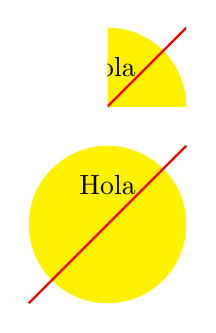
\begin{tikzpicture}
% Tambien podemos usar "clipping" para recortar. Eso si, hay que usarlo dentro de un entorno "scope" para evitar recortar todo el dibujo.
\begin{scope}
% Mostramos solo lo que este dentro de esta region que definimos con "clip".
\clip (0,0) rectangle (1,1);
\fill[yellow] (0,0) circle (1cm);

% Funciona con todo lo que pongamos, no solo fill
\draw[red, thick] (-1,-1) -- (1, 1);
\node at (0, 0.5) {Hola};
\end{scope}

% Vemos que pasa si ponemos lo mismo sin clipping.
\begin{scope}[yshift=-1.5cm] % Ventajas de scope: podemos mover una parte del dibujo con xshift/yshift. Tambien podriamos usar scale = 2 para doblarle el tamano, por ejemplo.
\fill[yellow] (0,0) circle (1cm);
\draw[red, thick] (-1,-1) -- (1, 1);
\node at (0, 0.5) {Hola};
\end{scope}
\end{tikzpicture}
\end{LTXexample}

\begin{LTXexample}[width=0.4\textwidth, pos=r]
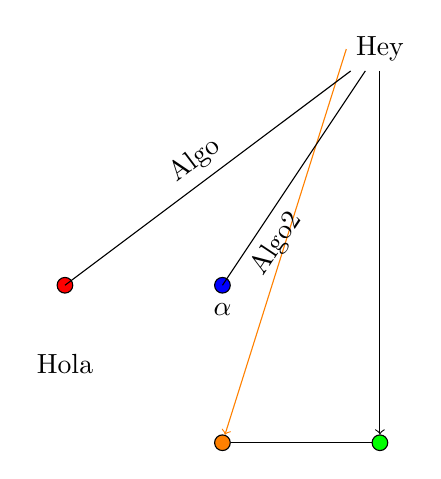
\begin{tikzpicture}
% Podemos poner nodos con texto o sin texto. Las llaves del final son necesarias siempre, eso si.
\node at (0, 1) {Hola};
\node[draw, circle, inner sep = 2pt, fill = red] at (0,2) {};

% Tambien se pueden poner etiquetas
\node[draw, circle, inner sep = 2pt, fill = blue, label = below:{$\alpha$}] at (2,2) {};

% Los nodos pueden ir nombrados para referenciarlos luego
\node[draw, circle, inner sep = 2pt, fill = orange] (A) at (2,0) {};
\node[draw, circle, inner sep = 2pt, fill = green] (B) at (4,0) {};
\draw (A) -- (B);

% Podemos hacerlo igual con los nodos con texto
\node (C) at (4, 5) {Hey};
\draw[->] (C) -- (B);

% Podemos decidir de que parte del nodo (south, west, north, east) sale la flecha
\draw[orange, ->] (C.west) -- (A);

% Y tambien podemos poner nodos en lineas
\draw (0,2) -- node[midway, above, sloped] {Algo} (C);
\draw (2,2) -- node[near start, below, sloped] {Algo2} (C);
\end{tikzpicture}
\end{LTXexample}

\begin{LTXexample}[width=0.4\textwidth, pos=r]
\usetikzlibrary{calc} % Para hacer calculos de puntos

\begin{tikzpicture}
% Dibujamos tres vertices de un triangulo
\node[draw, circle, inner sep = 2pt, fill = red, label = below:{$A$}] (A) at (0,0) {};
\node[draw, circle, inner sep = 2pt, fill = orange, label = below:{$B$}] (B) at (2.5,0) {};
\node[draw, circle, inner sep = 2pt, fill = green, label = above:{$C$}] (C) at (2,3) {};

% Ahora podemos hacer calculos y dibujar nodos donde queramos.
% Por ejemplo, un nodo a medio camino entre A y B
\node[draw, inner sep = 2pt, fill = blue] at ($(A)!0.5!(B)$) {};

% O sacar la recta perpendicular a AC que pasa por B
\draw (A) -- (C);
\draw[thick, dashed] (B) -- ($(A)!(B)!(C)$);

% Podemos sumar coordenadas
\node[draw, circle, inner sep = 2pt, fill = yellow, label = left:{$B + C$}] at ($(B) + (C)$) {};
\end{tikzpicture}
\end{LTXexample}

\begin{LTXexample}[width=0.4\textwidth, pos=r]

\begin{tikzpicture}
% Con colores tambien podemos hacer cosas chulas. Podemos combinarlos para sacar cosas distintas:
\fill[red!50!yellow] (0,0) rectangle (1,1);

% O hacer degradados
\fill[left color = red, right color = yellow] (2,0) rectangle (3,1);

% Y transparencias
\node at (4.5, 0.5) {Hola};
\fill[left color = red, right color = yellow, opacity = 0.3] (4,0) rectangle (5,1);
\end{tikzpicture}
\end{LTXexample}

\index{pgfplots}
\begin{LTXexample}[width=0.4\textwidth, pos=r]
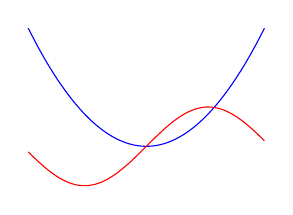
\begin{tikzpicture}
% Tambien podemos hacer funciones
\draw[scale=0.5,domain=-3:3,smooth,variable=\x,blue] plot ({\x},{\x*\x / 3});
\draw[scale=0.5,domain=-3:3,smooth,variable=\x,red] plot ({\x},{sin(\x r)});
% Nota: los senos y cosenos tikz los trata con grados. Hay que poner la r para que convierta a radiantes.
\end{tikzpicture}

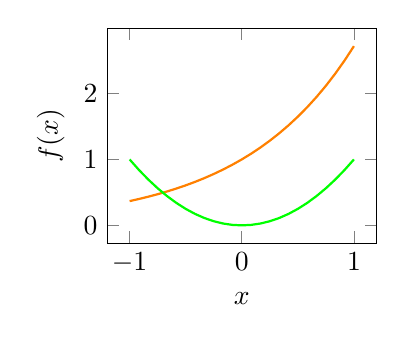
\begin{tikzpicture}
% Tambien se puede usar el entorno axis, que es mas facil de usar si solo queremos hacer graficas.
% Para activarlo, hay que poner \usepackage{pgfplots} en el preambulo.
\begin{axis}[width=5cm, domain = -1:1,	xlabel = $x$, ylabel = {$f(x)$}]
\addplot[color=orange, thick]{exp(x)};
\addplot[color=green, thick]{x^2};
\end{axis}
\end{tikzpicture}
\end{LTXexample}

\index{tikz-3dplot}
\index{3D}
\begin{LTXexample}[width=0.4\textwidth, pos=r]
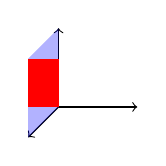
\begin{tikzpicture}
% Tikz tambien se maneja con coordenadas 3D
\draw[->] (0,0,0) -- (1,0,0);
\draw[->] (0,0,0) -- (0,1,0);
\draw[->] (0,0,0) -- (0,0,1);

% Aunque no del todo bien. Esto funciona
\fill[blue, opacity = 0.3] (0,0,0) -- (0,1,0) -- (0,1,1) -- (0,0,1) -- cycle;

% Pero esto no como queriamos
\fill[red] (0,0,0) rectangle (0,1,1);

% Para cosas en 3D mas avanzadas, ver
% tikz-3dplot
\end{tikzpicture}
\end{LTXexample}

\subsection{Un compilador más completo: latexmk}

\index{latexmk}
Al principio de este capítulo veíamos cómo funcionaba \LaTeX\ (\fref{sec:FuncionamientoLaTeX}), y que uno los problemas es que a veces hay que hacer varias pasadas para que funcione todo bien, lo cual puede ser un poco pesado. Por suerte, hay una solución llamada \textit{latexmk}, que es un compilador\footnote{En realidad es un script en Perl que llama a pdflatex y demás compiladores según convenga, pero para el caso es un compilador.} que se encarga de hacer todo esto de manera automática. Simplemente ejecutando \texttt{latexmk -pdf -silent documento.tex} compilará todo, haciendo tantas pasadas como haga falta.

La segunda ventaja de \textit{latexmk} es que nos permite compilar el documento de forma continua: cada vez que lo guardamos, \textit{latexmk} recoge los cambios y recompila para que nuestro lector de PDF pueda actualizar el documento\footnote{En Linux, Evince y Okular recargan el documento automáticamente. En OS X, Skim funciona muy bien.}. Para ello sólo tenemos que añadir el parámetro \textit{-pvc}: \texttt{latexmk -pdf -silent -pvc documento.tex}.

\textit{latexmk} tiene varias opciones más (ver su página de manual) y merece la pena probarlo y usarlo para quitarnos de problemas. Suele estar disponible como un paquete normal en las distribuciones Linux (\texttt{sudo apt-get install latexmk} funciona, por ejemplo) y también en MacPorts y Brew para OS X.

\subsection{Beamer: presentaciones con \LaTeX\ (o como dije adiós a Powerpoint)}

\section{Ampliando \LaTeX: Desarrollo de comandos, entornos, paquetes y clases}

\subsection{Comandos}

\subsection{Entornos}

\subsection{Paquetes y clases}

\subsection{Paquetes auxiliares para el desarrollo}
